\documentclass{beamer}
\usetheme{CambridgeUS}
%\usetheme{Madrid}
\usecolortheme{dolphin}
\title{Lecture 4}
\subtitle{Beamer presentation Example}
\author{Dr. Chenfei Zhang}
\date{\today}
\institute{UNNC}
\begin{document}
%*******************************************
\begin{frame}
\maketitle
\end{frame}
%*******************************************
\begin{frame}
\frametitle{Outlines}
\tableofcontents
\end{frame}

%*******************************************
\section{Introduction to Beamer}
%*******************************************3
\begin{frame}
``\underline{Frames}'' are the basic elements used in \textbf{beamer}.\\
\vfill

\pause % add slide transition

One frame $\ne$ One slide.\\

\pause

\vfill
The command \textbf{\textbackslash vfill} can adjust vertical spaces between different paragraphs within one frame.
\end{frame}
%*******************************************4
\begin{frame}
\frametitle{Basics}
In beamer documentclass, paragraphs, equations, lists, tables and figures can be typeset normally as in the \textbf{article} documentclass.\\[2ex]

\pause

While compiling the source codes, beamer will load common packages that are used for typesetting equations and figures, meaning we don't need to include the following packages in the preamble:
\begin{itemize}
\item
amsmath
\item
amssymb
\item
graphicx
\end{itemize}

\end{frame}
%*******************************************
\section{Old topics}
\subsection{Math envrionment}
%*******************************************
\begin{frame}
\frametitle{Math environment}

(Lab 1 Worksheet)\\
\[
\because x^{10} = 1024 \quad \therefore x=\pm 2
\]

\pause

(Lab 2 Worksheet)\\
\begin{equation}
\cos^2 \left(\frac{\theta}{2}\right) = \frac{1+\cos\theta}{2}
\end{equation}

\pause

\begin{eqnarray}
x+2y-z &=& 0 \nonumber \\
2x-3y+5z &=& 3 \\
-3y + 2z &=& -8
\end{eqnarray}

\end{frame}

%*******************************************
\subsection{Figure and Table}
%*******************************************
\begin{frame}
\frametitle{Figure}
Below is the plot of equation $x^3+y^3=3xy$ in \textbf{GeoGebra}.
\pause
\begin{figure}
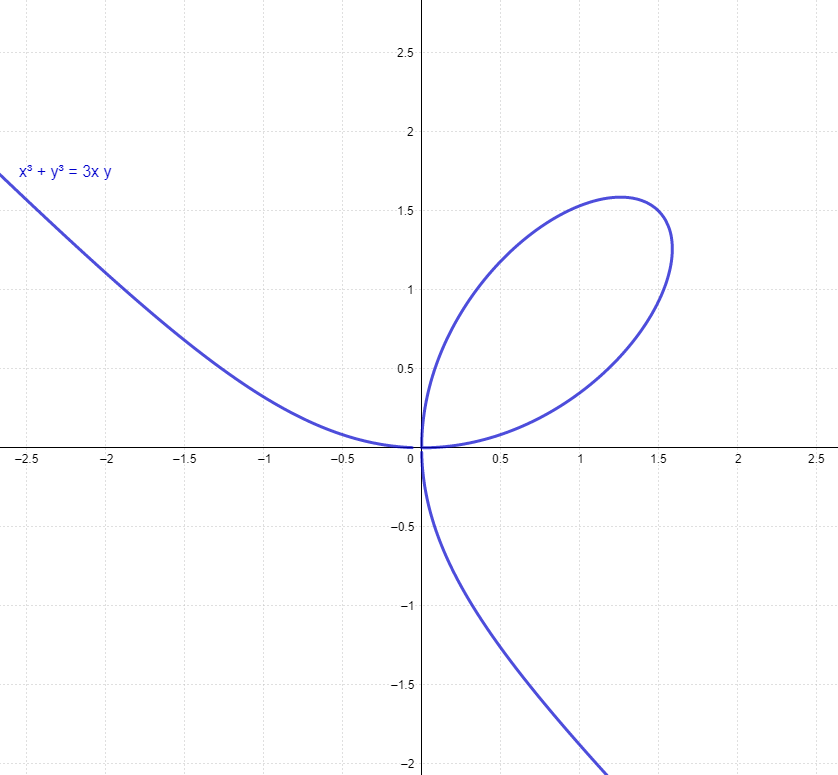
\includegraphics[scale=0.3]{eqnfig}
\caption{Folium of Descartes}
\label{fig1}
\end{figure}

\end{frame}

%*******************************************


\begin{frame}
\frametitle{Table}
(Lab 2 Worksheet)

\begin{table}
\centering
\caption{Time Complexity of Sorting Algorithms}
\begin{tabular}{|r|rr|}
\hline
Algorithm &  Average case & Best case \\
\hline
Insertion Sort & $O (n^2)$ & $O(n)$\\
Selection Sort & $O (n^2)$ & $O(n^2)$\\
Merge Sort & $O (n\log n)$ & $O(n\log n)$\\
Bubble Sort & $O (n^2)$ & $O(n)$\\
\hline
\end{tabular}
\end{table}

\end{frame}

%*******************************************
\section{New topics}
\subsection{Block environment}
%*******************************************
\begin{frame}
\frametitle{Block}

\begin{block}{A normal block}<1->
This is a block, normally used for highlighting the content within.
\end{block}

\begin{block}{Another normal block}<2->
Different beamer themes have different block styles and colors.
\end{block}

\vfill

\begin{alertblock}{This is an alertblock.}<3->
\textbf{Do not abuse blocks!}
\end{alertblock}


\end{frame}

%*******************************************
\subsection{Columns environment}
%*******************************************
\begin{frame}\label{frame1} % create label for later reference
\frametitle{Columns}
Here is a two-column example: equation on the left and figure on the right.\\
\vfill

\begin{columns} % start of two columns
\column{0.5\textwidth}<1-> % column 1
Differentiate both sides of $x^3+y^3 = 3xy$ w.r.t $x$:
\begin{eqnarray*}
3x^2+3y^2\frac{dy}{dx} &=& 3y+3x\frac{dy}{dx}\\
(3y^2-3x)\frac{dy}{dx}&=&3y-3x^2\\
\therefore \quad \frac{dy}{dx} &=& \frac{y-x^2}{y^2-x}
\end{eqnarray*}

\column{0.45\textwidth}<2-> % column 2
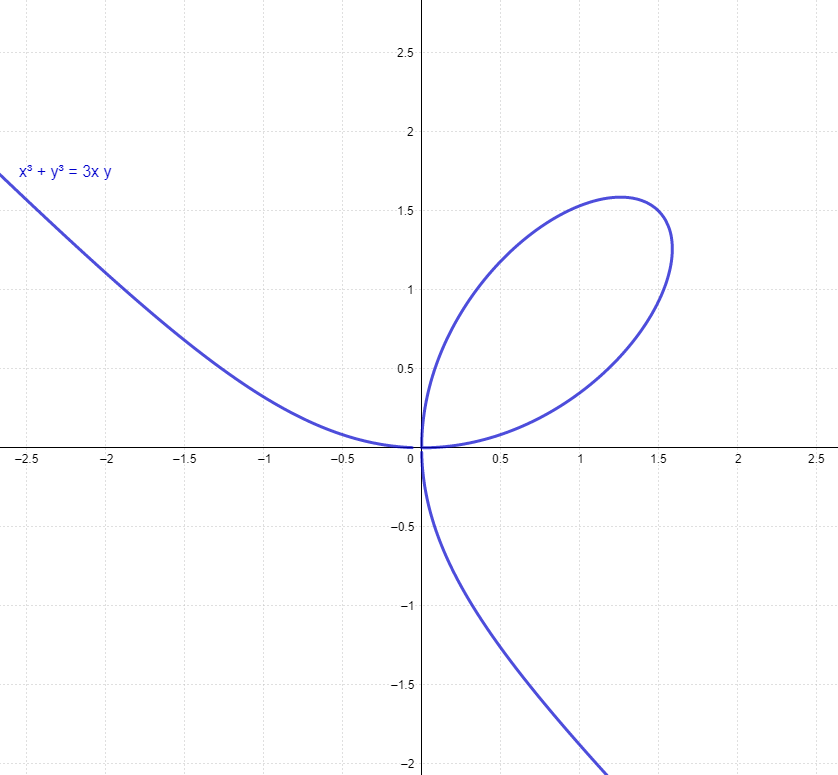
\includegraphics[scale=0.2]{eqnfig}
\end{columns} % end of two columns

\end{frame}

%*******************************************
\subsection{Verbatim environment}
%*******************************************
\begin{frame}[fragile] % [fragile] is need for verbatim
\frametitle{Verbatim}

To typeset the equation 
\[
x=\frac{-b\pm \sqrt{b^2-4ac}}{2a}
\]
we need the following command lines:\\
\pause
\begin{verbatim} 
\[
x=\frac{-b\pm \sqrt{b^2-4ac}}{2a}
\]
\end{verbatim} % lines above this command will appear exactly in the output
\pause
\begin{alertblock}{Note}
To use verbatim environment inside beamer frame, the optional setting \textbf{[fragile]} is needed (check the source code for this frame).
\end{alertblock}

\end{frame}
%*******************************************
\begin{frame}[fragile]
\frametitle{Verbatim}
Here is a two-column example: \LaTeX\,source code on the left and output on the right.\\[3ex]
\pause 
\begin{columns}
\column{0.45\textwidth} % column 1
Source code:\\
\begin{verbatim}
\begin{tabular}{c|l}
$p$ & $\sim p$  \\
\hline
T & F\\
F & T\\
\end{tabular}
\end{verbatim}
\pause 
\column{0.45\textwidth} % column 2
Output:\\[2ex]
\begin{tabular}{c|l}
$p$ & $\sim p$  \\
\hline
T & F\\
F & T\\
\end{tabular}
\end{columns}
\end{frame}

%*******************************************
\subsection{Hyperlink}
%*******************************************
\begin{frame}
\frametitle{Hyperlink}

Linking web addresses.\\
\begin{itemize}
\item
There are many good online tutorials for learning \LaTeX, for example, check \href{https://www.overleaf.com/learn/latex/Learn_LaTeX_in_30_minutes}{this link}.\\
\item
UNNC home page: \url{www.nottingham.edu.cn} 
\end{itemize}
\vspace{1cm}

\pause

Linking created labels.\\
\begin{itemize}
\item<2-> % add slide transition
Folium of Descartes is presented \hyperlink{fig1}{in this figure}.

\item<3-> % add slide transition
Check \hyperlink{frame1}{this frame} for implicit differentiation process.

\item<4-> % add slide transition
Check \hyperlink{frame1}{\beamerbutton{this frame}} for implicit differentiation process.
\end{itemize}


\end{frame}
%*******************************************



\end{document}